% This is samplepaper.tex, a sample chapter demonstrating the
% LLNCS macro package for Springer Computer Science proceedings;
% Version 2.20 of 2017/10/04
%
\documentclass[runningheads]{llncs}
%
\usepackage{graphicx}
\usepackage{longtable}
\graphicspath{ {./images/} }
% Used for displaying a sample figure. If possible, figure files should
% be included in EPS format.
%
% If you use the hyperref package, please uncomment the following line
% to display URLs in blue roman font according to Springer's eBook style:
% \renewcommand\UrlFont{\color{blue}\rmfamily}

\begin{document}
%
\title{Linear Algebra Assignment I}
%
%\titlerunning{Abbreviated paper title}
% If the paper title is too long for the running head, you can set
% an abbreviated paper title here
%
\author{Akash Panda {+91-9654659108}}
%
\authorrunning{Linear Algebra Assignment - I}
% First names are abbreviated in the running head.
% If there are more than two authors, 'et al.' is used.
%
\institute{Indian Institute of Science Bangalore, India\\
\email{akashpanda@iisc.ac.in}\\
\url{http://akashiisc.github.io}}
%
\maketitle              % typeset the header of the contribution
%
%
%
%
\section{Problem - I}
\subsection{Bonus question}
Yes, we can tell the maximum amount of potion that can be prepared out of the given ingredients. 
If we take each ingredient in maximum i.e. $m_1,m_2,m_3,m_4$, than the quantity of each according to various ratios being prepared would be maximum in total. 


\section{Problem - II}
\subsection{Second Part}
The time in below table is in seconds. 
\begin{longtable}{| p{.20\textwidth} | p{.20\textwidth} | p{.20\textwidth} |} 
\hline
Size of matrix & Time taken by Numpy implementation & Time talken by my Implementation\\
\hline
3 & 0.000607 & 0.000114 \\
4 & 0.000728 & 0.000188 \\
5 & 0.000646 & 0.000247 \\
6 & 0.000644 & 0.000375 \\
7 & 0.000683 & 0.000504 \\
8 & 0.000674 & 0.00071 \\
9 & 0.000714 & 0.000896 \\
10 & 0.000786 & 0.001198 \\
11 & 0.000803 & 0.001566 \\
12 & 0.000814 & 0.001878 \\
13 & 0.000807 & 0.002232 \\
14 & 0.000815 & 0.002758 \\
15 & 0.00087 & 0.003351 \\
16 & 0.000883 & 0.004015 \\
17 & 0.019521 & 0.007293 \\
18 & 0.024492 & 0.005709 \\
19 & 0.000938 & 0.005935 \\
20 & 0.000959 & 0.006843 \\
21 & 0.000934 & 0.007798 \\
22 & 0.001049 & 0.009011 \\
23 & 0.001011 & 0.010676 \\
24 & 0.001031 & 0.011573 \\
25 & 0.001071 & 0.012815 \\
26 & 0.001114 & 0.014194 \\
27 & 0.001101 & 0.019182 \\
28 & 0.001155 & 0.017298 \\
29 & 0.001341 & 0.021355 \\
30 & 0.001179 & 0.022208 \\
31 & 0.001617 & 0.024467 \\
32 & 0.001293 & 0.027317 \\
33 & 0.001248 & 0.029046 \\
34 & 0.001383 & 0.031659 \\
35 & 0.001388 & 0.034162 \\
36 & 0.005602 & 0.038022 \\
37 & 0.001468 & 0.040147 \\
38 & 0.001502 & 0.046256 \\
39 & 0.001465 & 0.047125 \\
40 & 0.001543 & 0.050121 \\
41 & 0.001548 & 0.053845 \\
42 & 0.001678 & 0.061607 \\
43 & 0.001664 & 0.066089 \\
44 & 0.002103 & 0.066367 \\
45 & 0.001876 & 0.072375 \\
46 & 0.001809 & 0.07655 \\
47 & 0.001843 & 0.085555 \\
48 & 0.001875 & 0.08573 \\
49 & 0.00218 & 0.097427 \\
50 & 0.001987 & 0.0953 \\
51 & 0.00197 & 0.100692 \\
52 & 0.002036 & 0.114387 \\
53 & 0.002084 & 0.125097 \\
54 & 0.002886 & 0.156338 \\
55 & 0.002758 & 0.16381 \\
56 & 0.00273 & 0.490499 \\
57 & 0.003634 & 0.478637 \\
58 & 0.003976 & 0.330869 \\
59 & 0.004812 & 0.201828 \\
60 & 0.003082 & 0.209823 \\
61 & 0.003162 & 0.220393 \\
62 & 0.00485 & 0.201896 \\
63 & 0.002757 & 0.214648 \\
64 & 0.008934 & 0.222989 \\
65 & 0.002881 & 0.2405 \\
66 & 0.00297 & 0.26233 \\
67 & 0.003086 & 0.254403 \\
68 & 0.003158 & 0.260414 \\
69 & 0.003198 & 0.273681 \\
70 & 0.003211 & 0.288618 \\
71 & 0.003354 & 0.306609 \\
72 & 0.00338 & 0.364858 \\
73 & 0.003907 & 0.372463 \\
74 & 0.005319 & 0.412921 \\
75 & 0.004027 & 0.406063 \\
76 & 0.004302 & 0.466005 \\
77 & 0.004197 & 0.464257 \\
78 & 0.004367 & 0.463425 \\
79 & 0.003622 & 0.411501 \\
80 & 0.004459 & 0.423162 \\
81 & 0.003892 & 0.437871 \\
82 & 0.003516 & 0.46641 \\
83 & 0.004218 & 0.525641 \\
84 & 0.003916 & 0.491401 \\
85 & 0.004281 & 0.619799 \\
86 & 0.004911 & 0.595451 \\
87 & 0.005017 & 0.613381 \\
88 & 0.005179 & 0.641346 \\
89 & 0.005381 & 0.676259 \\
90 & 0.005351 & 0.970028 \\
91 & 0.007573 & 1.091042 \\
92 & 0.007832 & 1.063807 \\
93 & 0.008227 & 0.944528 \\
94 & 0.006603 & 0.921807 \\
95 & 0.00728 & 0.940351 \\
96 & 0.006795 & 0.904228 \\
97 & 0.005947 & 0.853793 \\
98 & 0.006229 & 0.870714 \\
99 & 0.006324 & 0.920782 \\
\hline
\end{longtable}
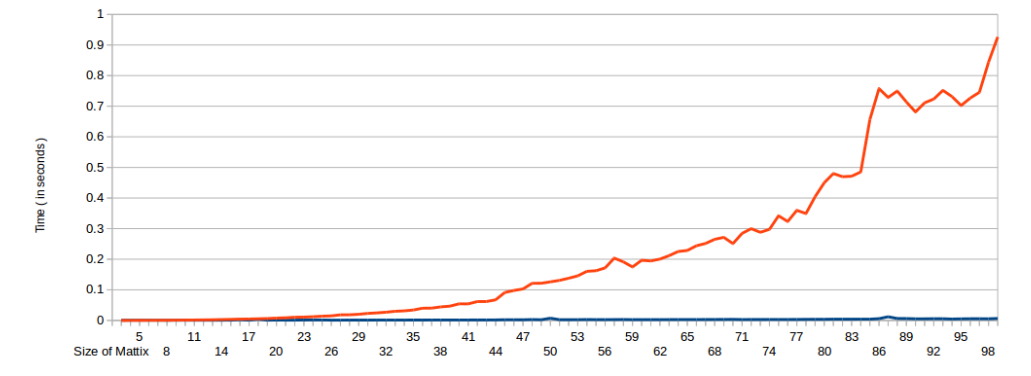
\includegraphics[scale=0.8]{profiling}
The red line in above figure denotes the time taken by My implementation of the inverse.\\
The blue line represents the time taken by the numpy implementation of the inverse.\\

As we can see from the table and figure above that upto very small matrices (size $\leq$7) my implementation was performing better. Then after that the time difference increased rapidly. We can conclude that the implementation is nowhere near the numpy.linalg.inv implementation of calculating inverse in performance. 

numpy.linalg.inv(A) calls numpy.linalg.solve(A,I) , where I is the identity matrix and solves using laplack's LU Factorization.~\cite{ref_proc1}

\subsection{Third Part}
Yes, We can find the inverse. We know that $(A^{-1})^T = (A^T)^{-1}$ 

Hence, if we convert the matrix A into its transpose. And the compute the inverse using the row operations. Then we will get inverse matrix of $A^T$.
As we know that this inverse matrix will be equal to $(A^{T})^{-1}$ , which will be again equal to $(A^{-1})^T$
So, if we calculate the transpose of it, we would get the matrix $A^{-1}$

So doing column operations is like executing row operations on the transpose of the matrix and then converting the inverse matrix to its transpose. 


\subsection{Bonus Question}
If we have only two out of the three operations at our disposal, we can explore the following possibilities:-
\begin{enumerate}
\item
We can construct the operation MULTIPLY using sub-operations.\\
"MULTIPLY C r1" will be same as "MULTIPLY AND ADD 1-C r1 r1"

In this case , we can see that a MULTIPLY operation is being converted to MULTIPLY AND ADD operation. There is not much difference in complexity of the operations. So there will not be any overhead in this case. 

\item
We can construct the operation SWAP using the following sub-operations.\\
Row1 -$>$ Row1 + Row2 : MULTIPLY 1 WITH Row2 AND ADD TO ROW1\\
Row2 -$>$ (-1)Row2 : MULTIPLY -1 with Row2 \\
Row2 -$>$ Row2 + Row1 : MULTIPLY 1 WITH Row1 AND ADD TO Row2\\
Row1 -$>$ Row1 - Row2 : MULTIPLY -1 WITH Row2 AND ADD TO Row1\\

In this case, we can see that there is much difference in complexity. A simple SWAP operation of 0(1) complexity is being converted into suboperations that require traversal of a complete row , now the complexity of the operation is O(x), where x is the number of columns. 

\end{enumerate}

%
% ---- Bibliography ----
%
% BibTeX users should specify bibliography style 'splncs04'.
% References will then be sorted and formatted in the correct style.
%
% \bibliographystyle{splncs04}
% \bibliography{mybibliography}
%
\begin{thebibliography}{1}
\bibitem{ref_proc1}
https://stackoverflow.com/questions/16569613/how-does-numpy-linalg-inv-calculate-the-inverse-of-an-orthogonal-matrix
\end{thebibliography}
\end{document}
